\chapter{Authentication Mechanisms}
\label{cha:authentication_mechanisms}
This chapter explains the concepts and mechanisms of the discussed authentication mechanisms.
Only the mTLS and and the JWT approach are discussed, since the TTN approach is deprecated and should not be used anymore~\cite{dias2020microservices}.
Furthermore this chapter clarifies the advantages and disadvantages of the discussed mechanisms.

\begin{figure}
	\centering
	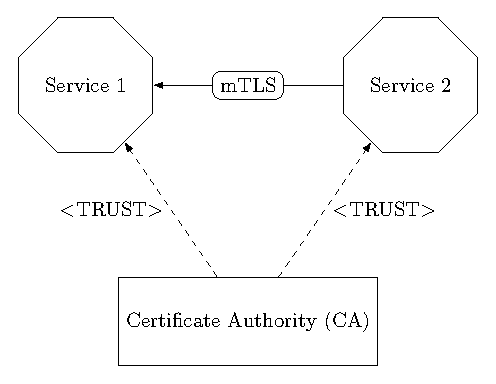
\includegraphics{images/authentication-mechanisms/TikZ_mTLS_base_structure.pdf}
	\caption{Setup using mTLS for the service-to-service authentication~\cite{dias2020microservices}}
	\label{fig:auth_mechanisms_mtls}
\end{figure}

\section{Authentication based on mTLS}
% TODO: Kurz erklären welchen Zusammenhang mtls mit Client Certificate Authentication hat
Mutual TLS is the most popular option for the service-to-service authentication of microservice deployments~\cite{dias2020microservices}.
Securing the communication with TLS already provides integrity, confidentiality and furthermore authenticates the server to the client.
Since basic TLS does not provide authentication from the client to the server, it is not sufficient for the service-to-service security.
Therefore mutual TLS is used, which provides an efficient and straightforward approach to authenticate the client to the server.

The authentication using mTLS requires a PKI, same as the authentication using basic TLS.
It is possible to use the already existing PKI of the internet, but this would make the key management much harder and would not bring any advantages.
% TODO: Insert Reference to self hosted PKI
Therefore it is good practise to use a self-hosted PKI to have a root of trust within the network~\cite{dias2020microservices}.
The setup of a microservice deployment using mTLS is shown in figure~\ref{fig:auth_mechanisms_mtls}.

When mTLS is used, both the server and the client must provide a valid certificate to create a communication channel.
The issuer of the presented certificates must be trusted by all communicating parties~\cite{dias2020microservices}.
If one communication partner does not have a valid certificate which is signed by a trusted issuer, the communication is neglected.
Therefore each service needs a private key, a public key.
Additionally a signed certificate, which binds the public key to the subject of the certificate, is needed.
The certificates of the communication partners are exchanged during the TLS handshake.

This mechanism can also be used to authenticate the end users of an application.
For this context the term Client Certificate Authentication (CCA) is used.
The service-to-service authentication using mTLS is a implementation of CCA, but in this approach the client is not the end user, instead it is another service.

\subsection{Handshake}
\label{sec:tlshandshake_details}
The handshake is used exchange to exchange the certificates of the participants and setup the connection.
The steps of the handshake differ between the used algorithms and versions of the TLS protocol.
The following sequence and figure~\ref{fig:tlshandshake} should give an overview about the steps of the TLS handshake using mutual TLS~\cite{parsovs2013practical}:
\begin{enumerate}
	\item The client initializes the connection by sending a \textbf{ClientHello} message to the server.
		The \textbf{ClientHello} message includes a list of supported cipher suits, and the randomness, which is a combination of random bytes and the current date~\cite{mediumtls}.
	\item The sever responds with a \textbf{ServerHello}, in which the server chooses one cipher suite of the \textbf{ClientHello} message.
		Furthermore the \textbf{ServerHello} contains the servers randomness.
	\item The server sends the \textbf{Certificate} messages, containing one or more certificates, which can be used to build the chain.
		The client validates the sent certificates with his own trusted store.
		If the trusts the sent certificate chain, the server is authenticated successfully.
	\item The server sends the \textbf{CertificateRequest} message, in which the trusted CAs of the server are listed.
		The client can use this list to choose the correct certificate he has to present.
	\item The server sends the \textbf{ServerHelloDone} message.
	\item The client responds with his \textbf{Certificate} message, which is similiar to the servers \textbf{Certificate} message, but contains the client's certificate.
	\item The client he generates a random value the pre-master secret, which is used to derive symmetric keys for the cipher suite.
		The pre-master secret is then encrypted, using the public key of the server.
		The public key of the server is assumed to be the first certificate of the \textbf{Certificate} message by the server.
		The encrypted pre-master secret is then transferred to the server within the \textbf{ClientKeyExchange} message.
	\item The client has to proove the client that he owns the corresponding private key of the sent certificate.
		Therefore he has to encrypt the hash of all previous messages with his private key.
		This encrypted hash is then sent to the server within the \textbf{CertificateVerify} message.
		The sever can decrypt the hash with the public key of the certificate and can calculate the hash on his own to check whether the decrypted hash is correct or not.
	\item The client sends a \textbf{ChangeCipherSpec} message, to signal the server, that all following messages will be protected with the protection mechanisms defined in the cipher suite.
	\item The last message of the handshake is the \textbf{Finished} message, which is an encrypted hash of all previous messages.
	\item Same as step 9, but from the server.
	\item Same as step 10, but from the server.
\end{enumerate}
After the handshake both participants know the secret, which can be used to encrypt and decrypt messages.
The handshake would have almost the same steps when mTLS is not used.
Only the \textbf{CertificateRequest} message of the sever and the \textbf{Certificate} message and the \textbf{CertificateVerify} message of the client are unique for mTLS.
One special case of the handshake is, that the client responds to the \textbf{CertificateRequest} with a empty \textbf{Certificate} message.
Depending on the configuration of the server, the connection without a certificates can be allowed or the connection will be aborted~\cite{parsovs2013practical}.

\begin{figure}
    \centering
	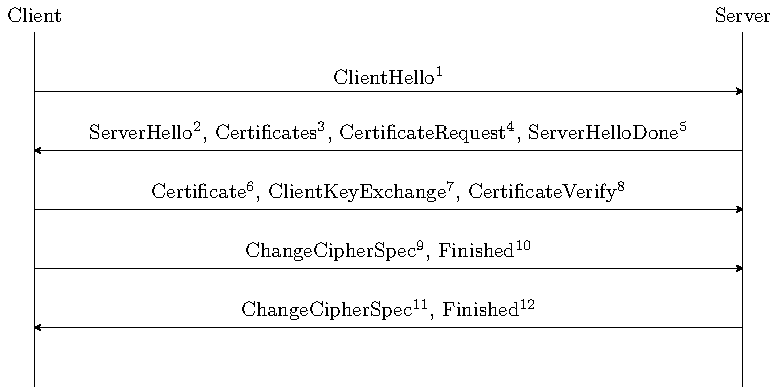
\includegraphics{authentication-mechanisms/TikZ_handshake.pdf}
    \caption{TLS handshake using mTLS~\cite{parsovs2013practical}}
	\label{fig:tlshandshake}
\end{figure}

%\begin{figure}
%    \centering
%	\begin{tikzpicture}
%		\draw (-6,0) -- (-6,-6) (6,0) -- (6,-6);
%		\node at (-6,.3) {Client};
%		\node at (6,.3) {Server};
%
%		\draw[-stealth] (-6,-1) -- node[midway,above] {ClientHello} (6,-1);
%		\draw[stealth-] (-6,-2) -- node[midway,above] {ServerHello, Certificate, CertificateRequest, ServerHelloDone} (6,-2);
%		\draw[-stealth] (-6,-3) -- node[midway,above] {Certificate, ClientKeyExchange, CertificateVerify} (6,-3);
%		\draw[-stealth] (-6,-4) -- node[midway,above] {ChangeCipherSpec, Finished} (6,-4);
%		\draw[stealth-] (-6,-5) -- node[midway,above] {ChangeCipherSpec, Finished} (6,-5);
%	\end{tikzpicture}
%    \caption{TLS handshake using mTLS~\cite{parsovs2013practical}}
%    \label{fig:tlshandshake}
%\end{figure}

\subsection{Passing the end user context}
For some functionalities, the identity of the microservice is not relevant, instead the identity of the end user is relevant.
In those cases, the microservices have to pass the end user context, when they consume the logic of other microservices.
The most popular approach for passing the end user context with mTLS are JSON Web Tokens.
This approach can be implemented in multiple ways~\cite{dias2020microservices}.

Genereally, the user obtains a access token from any token service.
This token could be a OAuth2 or a OpenID Connect token or any other token.
The user has to send this token with each request.
The token is than validated by a Security Token Service (STS).
If the token is valid, the STS returns a JWT, which can then be used to consume other services.
% TODO: Hurenkind
When one microservice calls another microservice he sends the JWT and if this microservice has to consume another microservice, he also passes the same token to the next microservice~\cite{dias2020microservices}.
This approach is shwon in figue~\ref{fig:mtls_id_1}
\begin{figure}
    \centering
	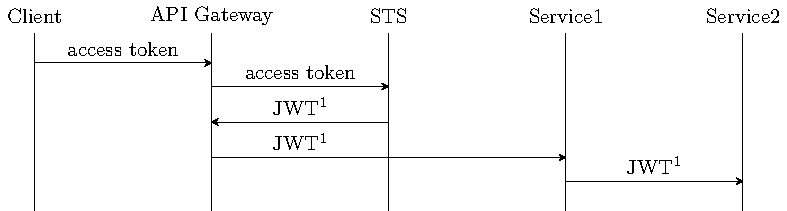
\includegraphics{images/authentication-mechanisms/TikZ_jwt_identity_1.pdf}
    \caption{Use the same JWT for each request~\cite{dias2020microservices}}
	\label{fig:mtls_id_1}
\end{figure}

Another approach is, that the STS is used to generate a new token for each request.
When the STS generates a new token for each request, he has full knowledge about all performed requests.
Therefore the STS could implement further authorization logic.
But the frequent calls could result in a enourmous workload for the STS and could decrease the performance of the whole system.
This approach is shwon in figue~\ref{fig:mtls_id_2}

\begin{figure}[H]
	\centering
	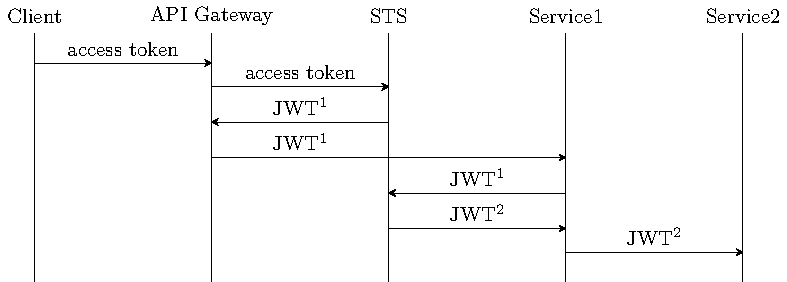
\includegraphics{images/authentication-mechanisms/TikZ_jwt_identity_2.pdf}
	\caption{Generate new JWT for each request~\cite{dias2020microservices}}
	\label{fig:mtls_id_2}
\end{figure}

Both approaches result in some overhead, especially the second approach, where a token has to be generated for each request.
Especially when the microservices are located in different trust domains, this can get very complicated, since a microservice only trusts the STS within his domain~\cite{dias2020microservices}.
Therefore, mTLS might not be the superior approach for systems, which require the services to know the end user context.

\subsection{Conclusion}
mTLS is a efficient mechanism to implement service to service authentication.
Since the communication between the services is usually done using HTTPS, the services already use TLS.
Therefore the use of mTLS does not cause much configuration overhead and no new technologies are necessary~\cite{dias2020microservices}, unless the services do not have to share the end user context between requests.

One crucial advantage of the TLS handshake is that the private keys are never exchanged and the session keys are always different, due to the usage of the randomness.
This means even if an intruder is able to get the session key of a communication channel, he is not able to use this key for another session.
Furthermore it is not possible to retrieve any information about the private key of the communication partners with the knowledge of the session key.
This shows how secure mTLS is, even for advanced attacks~\cite{parsovs2013practical}.

From the developer perspective, mTLS does not require to implement much logic.
The service which acts as the server has to be configured to use certificate authentication.
Depending on the used technologies, this is usually done by setting a few configuration parameters in the code, or directly on the webserver.
The service which acts as the client has to be configured to send his certificate during the TLS handshake.
Most HTTP Client libraries support to simply attach the certificate to each HTTP Request.
But the fact that the developers do not have to implement much logic, results in the problem, that they do not have much control about the system.
The developers have to rely on the implementation of the webserver developers.
This means if a webserver has security related bugs, the microservice developers can not solve them on their own.
For example the apache webserver, which is one of the most popular webservers had many issues, in combination with mTLS.
Arnis Parsovs~\cite{parsovs2013practical} researched about the problems of the apache webserver and gave an exhensive guide how to circumvent all bugs, when client certificate authentication is configured.

%The services of a microservice deployment usually host their APIs on webservers.
%Since microservice deployment's have multiple technology stacks, multiple different webservers might have to be used.
%The configuration of mTLS for a webserver is different from webserver to webserver.
%So the configuration has to be done multiple times, which results in a bigger attack surface.
%Especially because the mTLS implementations of the webservers might have bugs.
%Those bugs can be hard to fix, because the developers have to fully rely on the support of the webserver developers. 
%For example the apache webserver, which is one of the most popular webservers had many issues, in combination with mTLS.
%Resulting in many security risks, caused by wrong configurations~\cite{parsovs2013practical}. 

% TODO: Referenz auf key management
The biggest challenge of mTLS is the key management, which was described in more detail in chapter.
Key management is responsible for key provisioning, key revocation, key rotation and some more management tasks.
Usually the key management results in requiring a self-hosted PKI for the deployment.
For small applications the key management can be kept very simple.
But as soon as the deployment grows and many services are running at the same time, automation tools are required.
Therefore the management overhead of mTLS is much harder to handle, than the implementation of mTLS itself~\cite{dias2020microservices}.

The previous mentioned challenges and motivation result in the conclusion that mTLS is a very useful and efficient approach, when the developers do not require full control of the system.
Especially, when the end user context has to be shared among the services, mTLS might not be the most efficient solution.
Even if mTLS may not be the ultimate tool for all security challenges, in regard with service-to-service authentication, it does its job and it does it well.
This is the reason why mTLS is the most pupular approach for service-to-service authentication.

\section{Authentication based on self signed JWTs}
